\documentclass[aspectratio=169]{beamer}

% --- Tema Brown/MIT (exemplo, ajuste conforme instalação/localização) ---
\usetheme{Berlin}
\usecolortheme{mit}

\usepackage{tikz}

\usepackage{appendixnumberbeamer}

\usepackage{booktabs}
\usepackage[scale=2]{ccicons}

\usepackage{pgfplots}
\usepgfplotslibrary{dateplot}

\usepackage{xspace}
\newcommand{\themename}{\textbf{\textsc{metropolis}}\xspace}

\usepackage[backend=biber, style=authoryear]{biblatex}
\addbibresource{referencias.bib}

\iffalse
% --- CUSTOMIZAÇÃO DA CAPA ---
\setbeamertemplate{title page}
{%
  \begin{tikzpicture}[remember picture,overlay]
    % PDF de fundo (ocupa a página inteira)
    \node[at=(current page.center)] {
      
\includegraphics[width=\paperwidth,height=\paperheight]{fundo_capa.pdf}
    };

    % --- Texto em posições específicas ---
    % Título
    \node[anchor=west] at ([xshift=4.1cm,yshift=6.5     cm]current page.south west)
      {\usebeamerfont{title}\inserttitle};

    % Autor
    \node[anchor=west] at ([xshift=4.1cm,yshift=4.5cm]current page.south west)
      {\usebeamerfont{author}\insertauthor};

    % Data
    \node[anchor=west] at ([xshift=2cm,yshift=0.6cm]current page.south west)
      {\usebeamerfont{date}\insertdate};
  \end{tikzpicture}
}
\fi

% --- CUSTOMIZAÇÃO DA CAPA ---
\setbeamertemplate{title page}
{%
  \begin{tikzpicture}[remember picture,overlay]
    % PDF de fundo ocupa toda a página
    \node[at=(current page.center)] {
      
\includegraphics[width=\paperwidth,height=\paperheight]{fundo_capa.pdf}
    };

    % --- Texto em posições absolutas ---

    % Título
    \node[anchor=west,text width=0.45\paperwidth] 
      at ([xshift=4.1cm,yshift=6.5cm]current page.south west)
      {\usebeamerfont{title}\LARGE\textbf\inserttitle};

    % Autores
    \node[anchor=west,text width=0.6\paperwidth] 
      at ([xshift=4.1cm,yshift=4.5cm]current page.south west)
      {\usebeamerfont{author}\insertauthor};

    % Data
    \node[anchor=east] 
      at ([xshift=-0.8cm,yshift=2.0cm]current page.south east)
      {\usebeamerfont{date}\insertdate};

    % Centro/Núcleo
    \node[anchor=east,font=\bfseries] 
      at ([xshift=-0.8cm,yshift=1.2cm]current page.south east)
      {\insertinstitute};
  \end{tikzpicture}
}

% --- DADOS DO USUÁRIO ---
\title{Título da Pesquisa e/ou relatório elaborado}
\author{Autor 1\\
    Autor 2\\
    Autor 3\\
    Autor 4}
\date{24 de março, 2025}
\institute{Nome do centro/núcleo/iniciativa}

\iffalse
\pgfdeclareimage[height=0.5cm]{logo-insper-preto}{logo-insper-preto.pdf}
\logo{\pgfuseimage{logo-insper-preto}\hspace*{0.3cm}}

\AtBeginSection[]
{
  \begin{frame}<beamer>
    \frametitle{Conteúdo}
    \tableofcontents[currentsection]
  \end{frame}
}
\beamerdefaultoverlayspecification{<+->}
\fi

\pgfdeclareimage[height=0.5cm]{logo-insper-preto}{logo-insper-preto.pdf}
\logo{\pgfuseimage{logo-insper-preto}\hspace*{0.3cm}}

\AtBeginSection[]
{
  \begin{frame}<beamer>
    \frametitle{Conteúdo}
    \tableofcontents[currentsection]
  \end{frame}
}
\beamerdefaultoverlayspecification{<+->}

\begin{document}

% Slide de capa
\begin{frame}
  \titlepage
\end{frame}

\section{Introdução}

\begin{frame}{Objetivo da Apresentação}
    \begin{itemize}
        \item Demonstrar as principais funcionalidades do \texttt{beamer};
        \item Exibir elementos como listas, figuras, tabelas e equações;
        \item Referenciar bibliografia com Bib\LaTeX{}.
    \end{itemize}
\end{frame}

\section{Listas e Estruturas}

\begin{frame}{Exemplo de Lista Enumerada}
    \begin{enumerate}
        \item Primeiro item;
        \item Segundo item;
        \item Terceiro item.
    \end{enumerate}
\end{frame}

\begin{frame}{Lista em Blocos}
    \begin{block}{Bloco normal}
        Texto de exemplo em bloco.
    \end{block}
    \begin{alertblock}{Bloco de alerta}
        Destaque em vermelho.
    \end{alertblock}
    \begin{exampleblock}{Bloco de exemplo}
        Usado para exemplos práticos.
    \end{exampleblock}
\end{frame}

\section{Figuras e Tabelas}

\begin{frame}{Figura com TikZ}
    \centering
    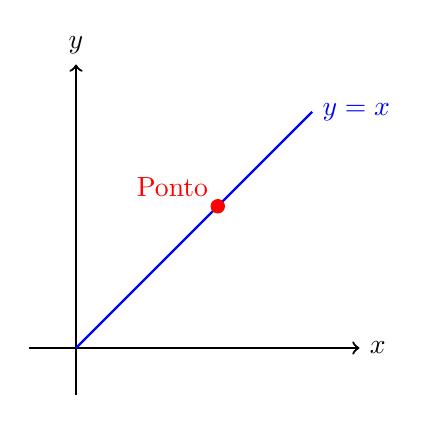
\begin{tikzpicture}[scale=1.2]
        \draw[thick,->] (-0.5,0) -- (3,0) node[right] {$x$};
        \draw[thick,->] (0,-0.5) -- (0,3) node[above] {$y$};
        \draw[blue,thick] (0,0) -- (2.5,2.5) node[right] {$y=x$};
        \filldraw[red] (1.5,1.5) circle (2pt) node[above left] {Ponto};
    \end{tikzpicture}
\end{frame}

\begin{frame}{Tabela de Exemplo}
    \centering
    \begin{tabular}{l|c|c}
        \textbf{Categoria} & \textbf{2024} & \textbf{2025} \\
        \hline
        A & 10 & 12 \\
        B & 20 & 22 \\
        C & 30 & 28 \\
    \end{tabular}
\end{frame}

\section{Equações}

\begin{frame}{Equações Matemáticas}
    Exemplo de equação inline: $y = ax + b$. \\[1em]

    Exemplo destacado:
    \[
        E = mc^2
    \]

    Exemplo de sistema:
    \[
        \begin{cases}
            x + y = 1 \\
            2x - y = 0
        \end{cases}
    \]
\end{frame}

\section{Referências Bibliográficas}

\begin{frame}{Citação no Texto}
    Podemos citar um livro clássico da economia \parencite{smith1776} 
    ou um artigo seminal em ciência de dados \parencite{breiman2001statistical}. 
\end{frame}

\begin{frame}[allowframebreaks]
    \frametitle{Referências}
    \printbibliography
\end{frame}

\end{document}